\documentclass[10pt,DIV16,a4paper,abstract=true,twoside=semi,openright]
{scrreprt}
\usepackage[USenglish]{babel}
\usepackage[numbers, sort&compress]{natbib}
\usepackage{isabelle,isabellesym}
\usepackage{booktabs}
\usepackage{paralist}
\usepackage{graphicx}
\usepackage{amssymb}
\usepackage{xspace}
\usepackage{xcolor}
\usepackage{hyperref}

\definecolor{lhWhite}        {RGB}{248,248,248}
\definecolor{lhBlack}        {RGB}{  8,  8,  8}
%
\definecolor{lhOrange}       {RGB}{243,107, 33}
\definecolor{lhGreen}        {RGB}{ 65,242, 34}
\definecolor{lhCyan}         {RGB}{ 34,169,242}
\definecolor{lhMagenta}      {RGB}{211, 34,242}
\definecolor{lhGold}         {RGB}{242,211, 34}
%
\definecolor{lhOrangeMedium} {RGB}{156, 69, 22}
\definecolor{lhGreenMedium}  {RGB}{ 42,156, 22}
\definecolor{lhCyanMedium}   {RGB}{ 22,109,156}
\definecolor{lhMagentaMedium}{RGB}{135, 22,156}
\definecolor{lhGoldMedium}   {RGB}{156,135, 22}
%
\definecolor{lhOrangeDark}   {RGB}{ 71, 31, 10}
\definecolor{lhGreenDark}    {RGB}{ 19, 71, 10}
\definecolor{lhCyanDark}     {RGB}{ 10, 50, 71}
\definecolor{lhMagentaDark}  {RGB}{ 62, 10, 71}
\definecolor{lhGoldDark}     {RGB}{ 51, 86, 28}
%
\definecolor{lhLightGray}    {RGB}{204,204,204}
\definecolor{lhDarkGray}     {RGB}{ 68, 68, 68}

\usepackage{dirtree}
\renewcommand*\DTstylecomment{\ttfamily\itshape}

\usepackage{ifthen}
\usepackage{lh-listings}
\usepackage{railsetup}

\sloppy

\pagestyle{headings}
\isabellestyle{default}
\setcounter{tocdepth}{1}
\newcommand{\ie}{i.\,e.\xspace}
\newcommand{\eg}{e.\,g.\xspace}
%\newcommand{\thy}{\isabellecontext}
%\renewcommand{\isamarkupsection}[1]{%
%  \begingroup% 
%  \def\isacharunderscore{\textunderscore}%
%  \section{#1 (\thy)}%
%  \def\isacharunderscore{-}%
%  \expandafter\label{sec:\isabellecontext}%
%  \endgroup% 
%}

\title{Automated Stateful Protocol Verification}
\author{%
\begin{minipage}{.8\textwidth}
  \centering
      \href{https://www.dtu.dk/english/service/phonebook/person?id=64207}{Andreas~V.~Hess}\footnotemark[1]
      \qquad\qquad
      \href{https://people.compute.dtu.dk/samo/}{Sebastian~M{\"o}dersheim}\footnotemark[1]
      \\
      \href{http://www.brucker.ch/}{Achim~D.~Brucker}\footnotemark[2]
      \qquad\qquad
      \href{https://people.cs.aau.dk/~andsch/}{Anders~Schlichtkrull}\footnotemark[3]
     \end{minipage}
}

\publishers{%
  \footnotemark[1]~DTU Compute, Technical University of Denmark, Lyngby, Denmark\texorpdfstring{\\}{, }
   \texttt{\{avhe, samo\}@dtu.dk}\\[2em]
  %
  \footnotemark[2]~
  Department of Computer Science, University of Exeter, Exeter, UK\texorpdfstring{\\}{, }
  \texttt{a.brucker@exeter.ac.uk}\\[2em]
  %
  \footnotemark[3]~
  Department of Computer Science, Aalborg University, Copenhagen, Denmark\texorpdfstring{\\}{, }
  \texttt{andsch@cs.aau.dk}
  %
}

\begin{document}
  \maketitle
  \begin{abstract}
    \begin{quote}
      In protocol verification we observe a wide spectrum from fully
      automated methods to interactive theorem proving with proof
      assistants like Isabelle/HOL.
      In this AFP entry, we present a fully-automated approach for
      verifying stateful security protocols, i.e., protocols with mutable
      state that may span several sessions.
      The approach supports reachability goals like secrecy and
      authentication.
      We also include a simple user-friendly transaction-based
      protocol specification language that is embedded into Isabelle.
      
    \bigskip
    \noindent{\textbf{Keywords:}} 
      Fully automated verification, stateful security protocols
    \end{quote}
  \end{abstract}


\tableofcontents
\cleardoublepage

\chapter{Introduction}
  In protocol verification we observe a wide spectrum from fully
  automated methods to interactive theorem proving with proof
  assistants like Isabelle/HOL. The latter provide overwhelmingly high
  assurance of the correctness, which automated methods often cannot:
  due to their complexity, bugs in such automated verification tools
  are likely and thus the risk of erroneously verifying a flawed
  protocol is non-negligible. There are a few works that try to
  combine advantages from both ends of the spectrum: a high degree of
  automation and assurance.

  Inspired by~\cite{brucker.ea:integrating:2009}, we present here a
  first step towards achieving this for a more challenging class of
  protocols, namely those that work with a mutable long-term state. To
  our knowledge this is the first approach that achieves fully
  automated verification of stateful protocols in an LCF-style theorem
  prover.  The approach also includes a simple user-friendly
  transaction-based protocol specification language embedded into
  Isabelle, and can also leverage a number of existing results such as
  soundness of a typed model (see,
  e.g.,~\cite{hess:typing:2018,hess.ea:formalizing:2017,hess.ea:typing:2018})
  and compositionality (see,
  e.g.,~\cite{hess:typing:2018,hess.ea:stateful:2018}). The Isabelle 
  formalization extends the AFP entry on stateful protocol composition and 
  typing~\cite{hess.ea:stateful:2020}.

  \begin{figure}
    \centering
    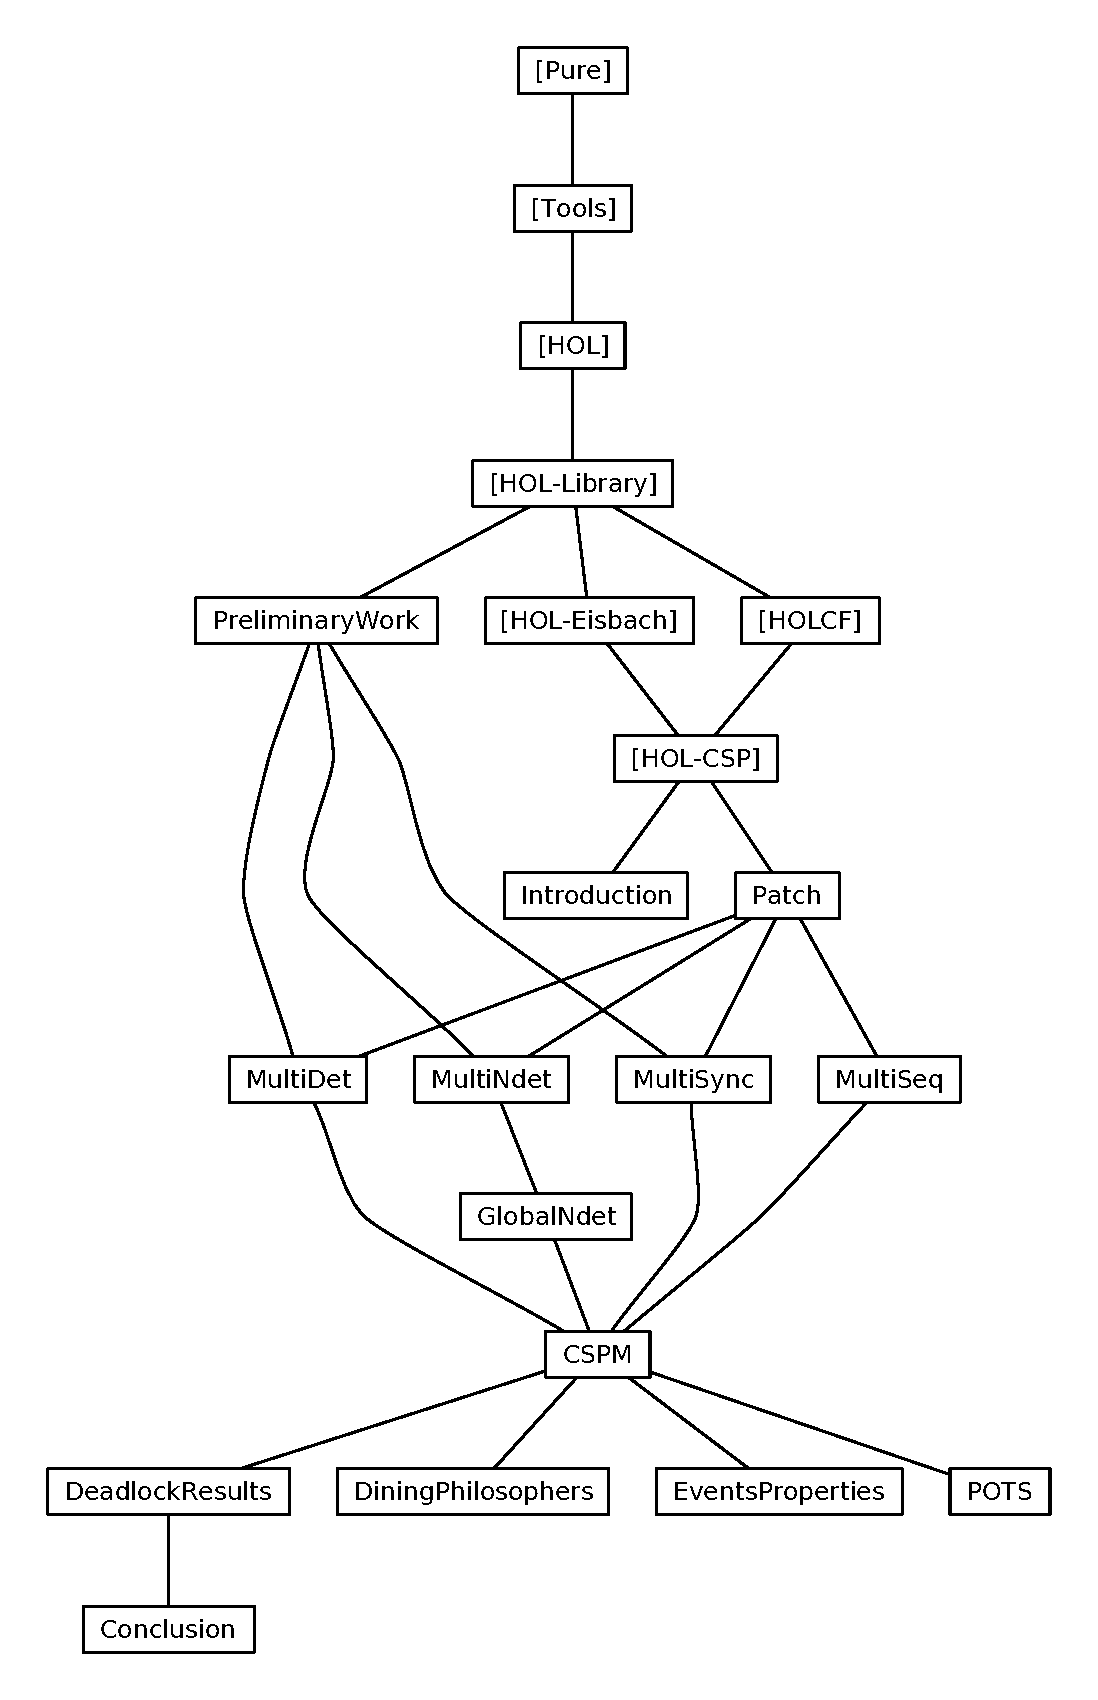
\includegraphics[height=\textheight]{session_graph}
    \caption{The Dependency Graph of the Isabelle Theories.\label{fig:session-graph}}
  \end{figure}
  The rest of this document is automatically generated from the
  formalization in Isabelle/HOL, i.e., all content is checked by
  Isabelle. \autoref{cha:manual} provides a manual of our automated protocol verification tool, called PSPSP, that is provided as part of this AFP entry. 
Thereafter, the structure of this document follows the
  theory dependencies (see \autoref{fig:session-graph}): After
  introducing the formal framework for verifying stateful security protocols
  (\autoref{cha:verification}), we continue with the setup for
  supporting the high-level protocol specifications language for
  security protocols (the Trac format) and the implementation of the
  fully automated proof tactics (\autoref{cha:trac}). Finally, we
  present examples (\autoref{cha:examples}).

\paragraph{Acknowledgments}
This work was supported by the Sapere-Aude project ``Composec: Secure Composition of Distributed Systems'', grant 4184-00334B of the Danish Council for Independent Research, by the EU H2020 project no. 700321 ``LIGHTest: Lightweight Infrastructure for Global Heterogeneous Trust management in support of an open Ecosystem of Trust schemes'' (lightest.eu) and by the ``CyberSec4Europe'' European Union's Horizon 2020 research and innovation programme under grant agreement No 830929.

\clearpage

\chapter{The PSPSP Manual}
\label{cha:manual}
\section{Motivation}
Because of its connected life, the modern world is increasingly
depending on secure implementations and configurations of network
infrastructures. As building blocks of the latter, firewalls are
playing a central role in ensuring the overall \emph{security} of
networked applications.

Firewalls, routers applying network-address-translation (NAT) and
similar networking systems suffer from the same quality problems as
other complex software. Jennifer Rexford mentioned in her keynote at
POPL 2012 that high-end firewalls consist of more than 20
million lines of code comprising components written in Ada as well as
LISP. However, the testing techniques discussed here are of
wider interest to all network infrastructure operators that need to
ensure the security and reliability of their infrastructures across
system changes such as system upgrades or hardware replacements. This
is because firewalls and routers are active network elements that can
filter and rewrite network traffic based on configurable rules. The
\emph{configuration} by appropriate rule sets implements a security
policy or links networks together.

Thus, it is, firstly, important to test both the implementation of a
firewall and, secondly, the correct configuration for each use. To
address this problem, we model firewall policies formally in
Isabelle/HOL. This formalization is based on the Unified Policy
Framework (UPF)~\cite{brucker.ea:upf:2014}. This formalization allows
to express access control policies on the network level using a
combinator-based language that is close to textbook-style
specifications of firewall rules. To actually test the implementation
as well as the configuration of a firewall, we use
HOL-TestGen~\cite{brucker.ea:interactive:2005,brucker.ea:hol-testgen-fw:2013,brucker.ea:theorem-prover:2012}
to generate test cases that can be used to validate the compliance of
real network middleboxes (e.g., firewalls, routers). In this document,
we focus on the Isabelle formalization of network access control
policies. For details of the overall approach, we refer the reader
elsewhere~\cite{brucker.ea:formal-fw-testing:2014}

\section{The Unified Policy Framework (UPF)}
Our formalization of firewall policies is based on the Unified Policy
Framework (UPF. In this section, we briefly introduce UPF, for all
details we refer the reader to)~\cite{brucker.ea:upf:2014}.

UPF is a generic framework for policy modeling with the primary goal
of being used for test case generation. The interested reader is
referred to~\cite{brucker.ea:model-based:2011} for an application of
UPF to large scale access control policies in the health care domain;
a comprehensive treatment is also contained in the reference manual
coming with the distribution on the \testgen website
(\url{http://www.brucker.ch/projects/hol-testgen/}).  UPF is based on
the following four principles:
\begin{enumerate}
\item policies are represented as \emph{functions} (rather than relations),
\item policy combination avoids conflicts by construction,
\item the decision type is three-valued (allow, deny, undefined),
\item the output type does not only contain the decision but also a
  `slot' for arbitrary result data.
\end{enumerate}


Formally, the concept of a policy is specified as a partial function
from some input to a decision value and additional some
output. \emph{Partial} functions are used because elementary policies
are described by partial system behavior, which are glued together by
operators such as function override and functional composition.
\begin{gather*}
  \types\enspace \alpha \mapsto \beta =
  \alpha \rightharpoonup \beta \operatorname{decision}
\end{gather*}
where the enumeration type $\operatorname{decision}$ is
\begin{gather*}
  \datatype \qquad \alpha\ap \operatorname{decision}
  = \operatorname{allow}\ap \alpha \mid
  \operatorname{deny}\ap \alpha
\end{gather*}

As policies are partial functions or `maps', the notions of a
\emph{domain} $\dom \ap p \ofType \alpha \rightharpoonup \beta
\Rightarrow \HolSet{\alpha}$ and a \emph{range} $\ran\ap p \ofType
[\alpha \rightharpoonup \beta] \Rightarrow \HolSet{\beta}$ can be
inherited from the Isabelle library.

Inspired by the Z notation~\cite{spivey:z-notation:1992}, there is the
concept of \emph{domain restriction} $\_ \triangleleft \_$ and
\emph{range restriction} $\_ \triangleright \_$, defined as:
\begin{gather*}
  \begin{array}{lrl}
    \isadefinition &\_ \triangleleft \_&\ofType \HolSet{\alpha}
           \Rightarrow \alpha \mapsto \beta \Rightarrow \alpha \mapsto \beta\\
    \where & S \triangleleft p &= \lambda x\spot \HolIf x \in S \HolThen p\ap x
    \HolElse \bottom \\[.5ex]
    \isadefinition & \_ \triangleright \_ &\ofType \alpha \mapsto
    \beta \Rightarrow \HolSet{\beta\ap\operatorname{decision}}
    \Rightarrow \alpha \mapsto \beta \\ 
    \where & p \triangleright S &= \lambda x\spot \HolIf
    \bigl(\operatorname{the}\ap
    (p\ap x)\bigr) \in S \HolThen p\ap x \HolElse \bottom \\
  \end{array}
\end{gather*}
The operator `$\operatorname{the}$' strips off the $\HolSome$, if it
exists. Otherwise the range restriction is underspecified.

There are many operators that change the result of applying the
policy to a particular element. The essential one is the
\emph{update}:
\begin{gather*}
  p(x \mapsto t) = \lambda y\spot \HolIf y = x \HolThen \lfloor
  t\rfloor \HolElse p\ap y
\end{gather*}

Next, there are three categories of elementary policies in UPF,
relating to the three possible decision values:
\begin{itemize}
\item The empty policy; undefined for all elements: $\emptyset =
  \lambda x\spot \bottom$
\item A policy allowing everything, written as $A_f\ap f$, or $A_U$ if
  the additional output is unit (defined as $\lambda x\spot \lfloor
  \operatorname{allow} ()\rfloor$).
\item A policy denying everything, written as $D_f\ap f$, or $D_U$ if
  the additional output is unit.
\end{itemize}

The most often used approach to define individual rules is to define a
rule as a refinement of one of the elementary policies, by using a
domain restriction. As an example,
\begin{gather*}
\bigl\{(\operatorname{Alice}, \operatorname{obj1},
\operatorname{read})\bigr\} \triangleleft A_U
\end{gather*}

Finally, rules can be combined to policies in three different ways:
\begin{itemize}
\item Override operators: used for policies of the same type, written
  as $\_ \oplus_i \_$.
\item Parallel combination operators: used for the parallel
  composition of policies of potentially different type, written as
  $\_ \otimes_i \_$.
\item Sequential combination operators: used for the sequential
  composition of policies of potentially different type, written as
  $\_ \circ_i \_$.
\end{itemize}

All three combinators exist in four variants, depending on how the
decisions of the constituent policies are to be combined. For example,
the $\_ \prodTwo \_$ operator is the parallel combination operator where the
decision of the second policy is used.

Several interesting algebraic properties are proved for UPF
operators. For example, distributivity
\begin{gather*}
( P_1 \oplus  P_2)  \otimes P_3  = ( P_1  \otimes P_3) \oplus ( P_2 \otimes P_3)
\end{gather*}
Other UPF concepts are introduced in this paper on-the-fly when
needed.


\input{KeyserverEx}
\input{manual}

\chapter{Stateful Protocol Verification}
\label{cha:verification}
\input{Transactions.tex}
\input{Term_Abstraction.tex}
\input{Stateful_Protocol_Model.tex}
\input{Term_Variants.tex}
\input{Term_Implication.tex}
\input{Stateful_Protocol_Verification.tex}

\chapter{Trac Support and Automation}
\label{cha:trac}
\input{Eisbach_Protocol_Verification.tex}
\input{ml_yacc_lib.tex}
\input{trac_term.tex}
\input{trac_fp_parser.tex}
\input{trac_protocol_parser.tex}
\input{trac.tex}

\chapter{Examples}
\label{cha:examples}
\input{Keyserver.tex}
\input{Keyserver2.tex}
\input{Keyserver_Composition.tex}
\input{PKCS_Model03.tex}
\input{PKCS_Model07.tex}
\input{PKCS_Model09.tex}

% \input{session}


{\small
  \bibliographystyle{abbrvnat}
  \bibliography{root}
}
\end{document}
\endinput 
%%% Local Variables:
%%% mode: latex
%%% TeX-master: t
%%% End:

